\section{Related Works}\label{sec:related}%
There have been several studies addressing the gender issue in Computer Science. Lagesen describes CS as STEM field that has excluded women~\cite{vivian_2007}. Putnik et al. presents data from Yugoslavia, comparing gender ratios and observing a higher number of men compared women~\cite{zoran_2017}.

Stout et al. in~\cite{jane_2016} and Cheryan et al. in~\cite{sappa_2013} provide studies about stereotyping in Computer majors, also arguing that there is a higher ratio of men than women in this field in the US. Likewise, Mercier et al. present surveys, drawings, and interviews which were used to examine the perception of US middle school students about characteristics of knowledgeable computer users~\cite{Mercier_2006}. These results showed cultural stereotypes of a computer user: 89\% were male and 94\% wore glasses.

Keinan et al. show data that the ratio of graduated women from Bachelor's programs in CS was of almost 40\% in 1984, dwindling to 20\% by 2006 in the US~\cite{keinan_2017}. Vardi has similar results, and adds that in 2013 and 2014, only 14.7\% of those graduates were women~\cite{moshe_2015}.

Papastergiou used descriptive statistics, principal component analysis and analysis of variance in~\cite{papastergiou_are_2008} to investigate 358 Greek high school students' intentions and motivation for pursuing academic studies in CS. This study looked into several factors, such as the influence of family and academic environment on their career choices, their perception of a professional career in CS, and their self-efficacy beliefs regarding computers. The analysis showed that a lack of exposure to and use of a computer at home and in school from early stages in the students' lives seems to be the main factor in discouraging them from studying CS, specially considering the data for girls.

Anderson et al. applied means, \mbox{Mann-Whitney} $U$ test comparison, and non-parametric statistics in~\cite{anderson_because_2008} to study possible factors related to low rates of female participation in education pathways leading to information and communications technology (ICT) professions, considering data from a three-year period. The survey had binary options, such as ``I am very interested in computers'' and ``I am not interested in computers'', was presented to 1,453 high school girls in their Senior year. The study identified two factors associated with a woman's aversion to ICT careers: the perception that the subject is boring, and an intense dislike of computers.

Maia describes a similar situation in~\cite{maia_2016}, presenting a study on female participation in university majors in CS in Brazil, based on the Higher Education Census data from the Ministry of Culture and Education between the years of 2000 and 2013. One of the issues raised was that while the number of male graduates increased 98\% in the period, that of female graduates decreased 8\%.

The Department of Computer Science\footnote{\url{http://cic.unb.br}} at the University of Brasília (UnB) currently offers three undergraduate degrees related to CS: Bachelor of Computer Science (since 1987), Licentiate in Computing (since 1997), and Computer Engineer (since 2008). Figure~\ref{fig:computerMajorUnB} shows gender data for students enrolled in them.

\begin{figure}%
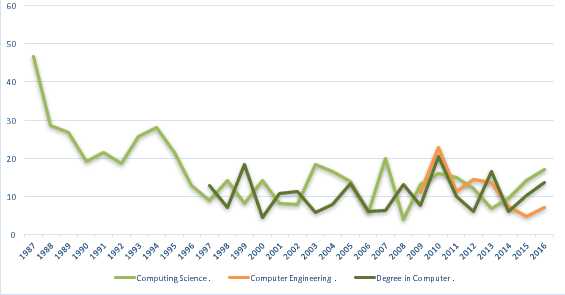
\includegraphics[width=\textwidth]{img/Figure1-girlsUnB}%
\caption{Ratio of female students enrolled in UnB's CS majors.}%
\label{fig:computerMajorUnB}%
\end{figure}%

In 1987, when the Bachelor course began, the gender difference between students enrolled was relatively low: 47\% of were female. However, this number decreased over time and, in 1997, this percentage fell to 10\%; by 2013 it was only 6\%. The Licentiate degree's ratio oscillates roughly around 11\%, while the Computer Engineer, which already began with low numbers, saw them fall to less than 12\% in the past three years.

We can see from the data that the difference between the number of male and female students enrolled in a CS major at UnB has decreased over the years, similar to what was reported in the before mentioned surveys. Given this alarming decline, and the widening disparity between male and female representations in the field of Computer Science, our work aims to investigate possible reasons for such scenario.\gnramos{Acho que poderia ficar explícito o porque da necessidade de mais mulheres. (``o que a diversidade acrescenta?'' e o que poderia ser feito com os resultados para melhorar a situação)}
